%%%%%%%%%%%%%%%%%%%%%%%%%%%%%%%%%%%%%%%%%%%%%%%%%%%%%%%%%%%%%%%%%%
% Sample template for MIT Junior Lab Student Written Summaries
% Available from http://web.mit.edu/8.13/www/Samplepaper/sample-paper.tex
%
% Last Updated August 30, 2011
%
% Adapted from the American Physical Societies REVTeK-4.1 Pages
% at http://publish.aps.org
%
% ADVICE TO STUDENTS: Each time you write a paper, start with this
% template and save under a new filename. If convenient, don't
%    erase unneeded lines, just comment them out.  Often, they
%    will be useful containers for information.
%
% Using pdflatex, images must be either PNG, GIF, JPEG or PDF.
%     Turn eps to pdf using epstopdf.
%%%%%%%%%%%%%%%%%%%%%%%%%%%%%%%%%%%%%%%%%%%%%%%%%%%%%%%%%%%%%%%%%%


%%%%%%%%%%%%%%%%%%%%%%%%%%%%%%%%%%%%%%%%%%%%%%%%%%%%%%%%%%%%%%%%%%
% PREAMBLE
% The preamble of a LaTeX document is the set of commands that precede
% the \begin{document} line.  It contains a \documentclass line
% to load the REVTeK-4.1 macro definitions and various \usepackage
% lines to load other macro packages.
%
% ADVICE TO STUDENTS: This preamble contains a suggested set of
% class options to generate a ``Junior Lab'' look and feel that
% facilitate quick review and feedback from one's peers, TA's
% and section instructors. Don't make substantial changes without
%     first consulting your section instructor.
%%%%%%%%%%%%%%%%%%%%%%%%%%%%%%%%%%%%%%%%%%%%%%%%%%%%%%%%%%%%%%%%%%

\documentclass[aps,twocolumn,secnumarabic,balancelastpage,amsmath,amssymb,nofootinbib]{revtex4}
%\documentclass[aps,twocolumn,secnumarabic,balancelastpage,amsmath,amssymb,nofootinbib]{revtex4-1}
\pdfpagewidth 8.5in
\pdfpageheight 11in

\usepackage{lgrind} % convert program listings to a form includable in a LaTeX document
\usepackage{chapterbib} % allows a bibliography for each chapter(each labguide has it's own)
\usepackage{color} % produces boxes or entire pages with coloredbackgrounds
\usepackage{graphics}      % standard graphics specifications
\usepackage[pdftex]{graphicx} % alternative graphics specifications
\usepackage{longtable}     % helps with long table options
\usepackage{epsf} % old package handles encapsulated post scriptissues
\usepackage{bm}            % special 'bold-math' package
%\usepackage{asymptote} % For typesetting of mathematical illustrations
\usepackage{thumbpdf}
\usepackage[colorlinks=true]{hyperref} % this package should be added after all others
% use as follows: \url{http://web.mit.edu/8.13}
\usepackage{multirow}
\usepackage{subfigure}

% Define a useful new command for writing units
\newcommand{\cd}{$\cdot$}

%
% And now, begin the document...
%

\begin{document}
\title{M{\"o}ssbauer Spectroscopy in $^{57}Fe$ Compounds}
\author{Jay M.\ Lawhorn}
\email{klawhorn@mit.edu}
\date{\today}
\affiliation{MIT Department of Physics}

\begin{abstract}

\end{abstract}

\maketitle

%\begin{figure}[htb]
%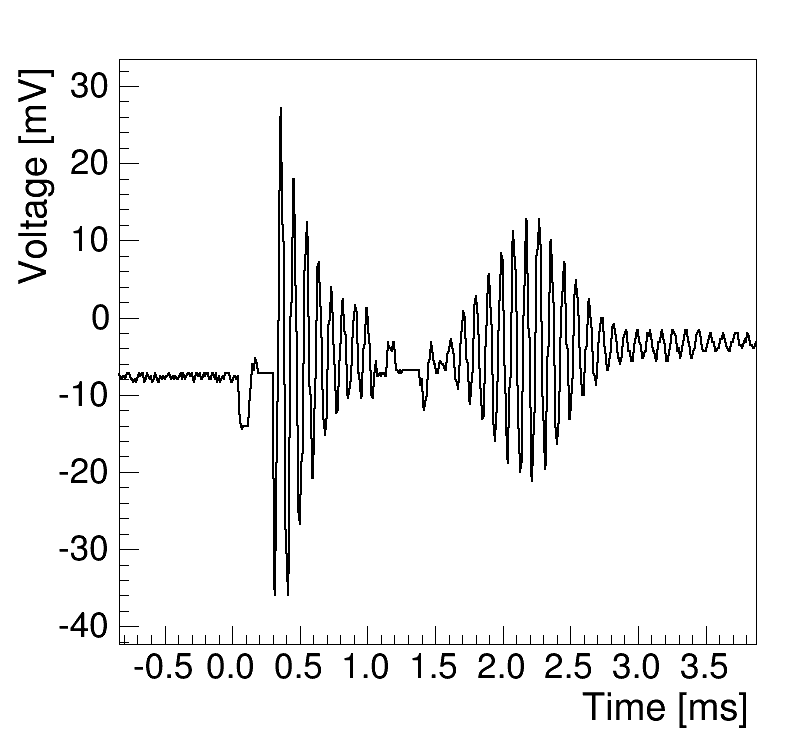
\includegraphics[width=6cm]{water_n2/fidecho.png}
%\caption{caption}
%\label{fig:fidecho}
%\end{figure}

\section{Introduction}

When an excited nucleus emits a gamma ray to transition to a lower state, the nucleus must recoil from the emission to conserve momentum. The energy of the gamma ray is then equal to the transition energy less the kinetic energy gained by the recoilling nucleus. Similarly, transition to the higher state requires a more energetic gamma ray than the true transition energy. A gamma ray emitted in this regime is unlikely to be energetic enough to excite the reverse transition in an identical nucleus.

When the excited nucleus is embedded in a lattice structure, the entire lattice recoils against the emitted gamma ray. Because the lattice is much more massive than a single nucleus, the kinetic energy imparted to the lattice is negligible compared to the energy of the gamma ray. Nuclear resonant absorption is thus much more likely to occur because the emitted gamma ray has energy much closer to the true transition energy. 

Recoilless nuclear resonance absorption of gamma radiation is known as the M{\"o}ssbauer effect and is used for ultra-high resolution spectroscopy with resolution $\Delta E/E\approx10^{12}$.

natural line width associated with lifetime of excited state by uncertainty principle, low-energy nuclear excited states are shortlived and therefore produce very sharp peaks

line widths broadened by thermal excitations in source/absorber

\section{Apparatus}

The apparatus consists of a specially prepared M{\"o}ssbauer source mounted on an oscillating piston, a proportional gas counter, and an absorber placed between the two. The M{\"o}ssbauer source is $^{57}_{27}$Co diffused in a platinum substrate that allows recoilless emission of 14.4 keV photons. 

\section{$^{57}Fe$ Zeeman splittings}

\section{Absolute Velocity Calibration}

\section{Zeeman and Quadrupole effects in $Fe_{2}O_{3}$}

\section{Magnetite}

\section{Line Broadening}

\begin{table}[h]
\caption{\label{table}}
\begin{tabular}{|c|c|c|}
\hline
Parameter & System & Value \\
\hline
g$_1$ & $^{57}$Fe & $(1.21\pm0.04)\times 10^{-7}$ eV \\
\hline
g$_0$ & $^{57}$Fe & $(2.13\pm0.05)\times 10^{-7}$ eV \\
\hline
$\mu_1 / \mu_0$ & $^{57}$Fe & $-1.71\pm0.07$ \\
\hline
g$_1$ & $Fe_2 O_3$ & $(1.91\pm0.06)\times 10^{-7}$ eV \\
\hline
g$_0$ & $Fe_2 O_3$ & $(3.34\pm0.06)\times 10^{-7}$ eV\\
\hline
q & $Fe_2 O_3$ & $(6\pm9)\times 10^{-9}$ eV\\
\hline
$\mu_1 / \mu_0$ & $Fe_2 O_3$ & $-1.71\pm0.06$ \\
\hline
\end{tabular}
\end{table}

\begin{thebibliography}{3}

\bibitem{crc}
	"Nuclear Spins, Moments, and Other Data related to NMR Spectroscopy" from \emph{Handbook of Chemistry and Physics},
	94th ed.,
	2013.

\bibitem{ray}
	R. Freeman,
	"Spin-Lattice Relaxation" from \emph{A Handbook of Nuclear Magnetic Resonance},
	Longman,
	1988.

\bibitem{blo}
	N. Bloembergen,
	"Nuclear Magnetic Relaxation" reprinted in \emph{Nuclear Magnetic Relaxation},
	W.A. Benjamin,
	1961.

\end{thebibliography}

\end{document}
